\newpage
\section{Questão 12-20}

\begin{figure}[H]
	\centering
	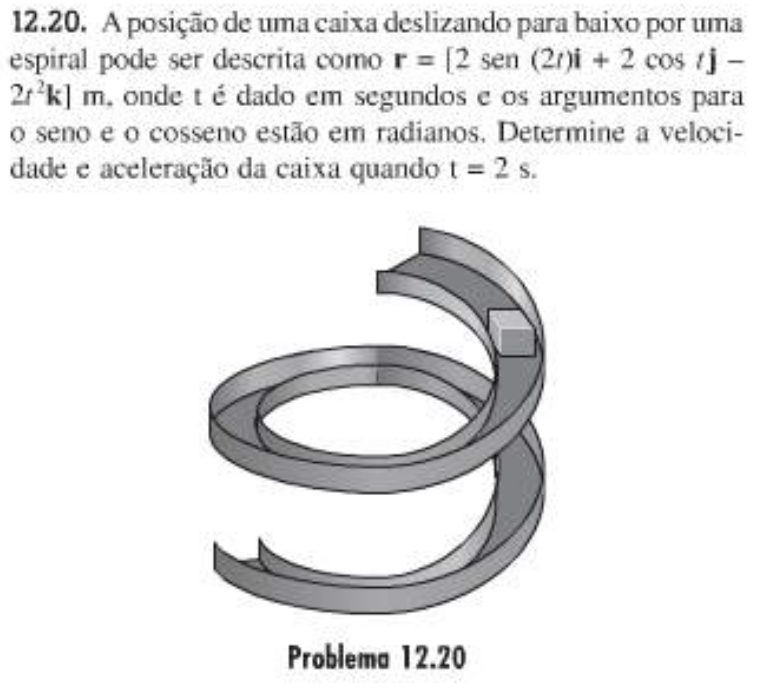
\includegraphics[width=0.7\linewidth]{fundamentais/12-20.png}
	\caption{Comando da questão 12-20.}\label{fig:q12-20}
\end{figure}

Nesta questão, analisamos a posição, velocidade e aceleração de uma partícula cujo movimento é descrito por uma função vetorial em um espaço tridimensional. Determinamos as expressões para a velocidade e aceleração vetoriais e avaliamos seus valores numéricos no instante \(t = 2 \, \text{s}\).

\subsection*{Função Vetorial da Posição}
A posição da partícula é descrita pela função vetorial:
\[
\vec{r}(t) = 2 \sin(2t) \, \hat{i} + 2 \cos(t) \, \hat{j} - 2t^2 \, \hat{k},
\]
onde:
\begin{itemize}
    \item \(\hat{i}, \hat{j}, \hat{k}\) são os vetores unitários nas direções \(x\), \(y\) e \(z\), respectivamente;
    \item \(t\) é o tempo.
\end{itemize}

\subsection*{Velocidade Vetorial}
A velocidade da partícula é obtida pela derivada de \(\vec{r}(t)\) em relação ao tempo:
\[
\vec{v}(t) = \frac{d\vec{r}(t)}{dt}.
\]

Calculando cada componente:
\[
\vec{v}(t) = 4 \cos(2t) \, \hat{i} - 2 \sin(t) \, \hat{j} - 4t \, \hat{k}.
\]

\subsection*{Aceleração Vetorial}
A aceleração da partícula é obtida pela derivada de \(\vec{v}(t)\) em relação ao tempo:
\[
\vec{a}(t) = \frac{d\vec{v}(t)}{dt}.
\]

Calculando cada componente:
\[
\vec{a}(t) = -8 \sin(2t) \, \hat{i} - 2 \cos(t) \, \hat{j} - 4 \, \hat{k}.
\]

\subsection*{Valores Numéricos no Instante \(t = 2 \, \text{s}\)}
Substituímos \(t = 2 \, \text{s}\) nas expressões de \(\vec{v}(t)\) e \(\vec{a}(t)\) para calcular seus valores numéricos:

\[
\vec{v}(2) = 4 \cos(4) \, \hat{i} - 2 \sin(2) \, \hat{j} - 8 \, \hat{k}.
\]

\[
\vec{a}(2) = -8 \sin(4) \, \hat{i} - 2 \cos(2) \, \hat{j} - 4 \, \hat{k}.
\]

\subsection*{Resultados Finais}
\begin{itemize}
    \item Velocidade vetorial:
    \[
    \vec{v}(t) = 4 \cos(2t) \, \hat{i} - 2 \sin(t) \, \hat{j} - 4t \, \hat{k}.
    \]
    Valor no instante \(t = 2 \, \text{s}\):
    \[
    \vec{v}(2) = 4 \cos(4) \, \hat{i} - 2 \sin(2) \, \hat{j} - 8 \, \hat{k} = -2.614 \,\hat{i} + 1.8185 \,\hat{j} - 8\,\hat{k}
    \]

    \item Aceleração vetorial:
    \[
    \vec{a}(t) = -8 \sin(2t) \, \hat{i} - 2 \cos(t) \, \hat{j} - 4 \, \hat{k}.
    \]
    Valor no instante \(t = 2 \, \text{s}\):
    \[
    \vec{a}(2) = -8 \sin(4) \, \hat{i} - 2 \cos(2) \, \hat{j} - 4 \, \hat{k} = 6.0544 \,\hat{i} + 0.8323 \,\hat{j} - 4\,\hat{k}
    \]
\end{itemize}
